\chapter{Выполнение лабораторной работы}

\section{Индивидуальное задание}

\textbf{Вариант 1 (19)}

Сетевой коммутатор на 128 портов. Сформировать в хост-подсистеме и передать в SPE таблицу коммутации из 254 ip адресов 195.19.32.1/24 (адреса 195.19.32.1 .. 195.19.32.254). Каждому адресу поставить в соответствие один из 128 интерфейсов (целые числа 0..127). Выполнить тестирование работы коммутатора, посылая из хост-подсистемы ip адреса и сравнивая полученный от GPC номер интерфейса с ожидаемым.




\section{Код программы}

\captionsetup{singlelinecheck = false, justification=raggedright}
\begin{lstlisting}[label=full, caption=sw\_kernel\_main.c]
#include <stdlib.h>
#include <unistd.h>
#include "lnh64.h"
#include "gpc_io_swk.h"
#include "gpc_handlers.h"

#define SW_KERNEL_VERSION 26
#define DEFINE_LNH_DRIVER
#define DEFINE_MQ_R2L
#define DEFINE_MQ_L2R
#define __fast_recall__

#define TEST_STRUCTURE 1

extern lnh lnh_core;
extern global_memory_io gmio;
volatile unsigned int event_source;

int main(void) {
	//Leonhard driver structure should be initialised
	lnh_init();
	//Initialise host2gpc and gpc2host queues
	gmio_init(lnh_core.partition.data_partition);
	for (;;) {
		//Wait for event
		while (!gpc_start());
		//Enable RW operations
		set_gpc_state(BUSY);
		//Wait for event
		event_source = gpc_config();
		switch(event_source) {
			case __event__(insert_burst) : insert_burst(); break;
			case __event__(search_burst) : search_burst(); break;
		}
		//Disable RW operations
		set_gpc_state(IDLE);
		while (gpc_start());
		
	}
}

void insert_burst() {
	lnh_del_str_sync(TEST_STRUCTURE);
	unsigned int count = mq_receive();
	unsigned int size_in_bytes = 2*count*sizeof(uint64_t);
	uint64_t *buffer = (uint64_t*)malloc(size_in_bytes);
	buf_read(size_in_bytes, (char*)buffer);
	for (int i=0; i<count; i++) {
		lnh_ins_sync(TEST_STRUCTURE,buffer[2*i],buffer[2*i+1]);
	}
	lnh_sync();
	free(buffer);
}

void search_burst() {
	lnh_sync(); 
	unsigned int count = lnh_get_num(TEST_STRUCTURE);
	mq_send(count);
	auto key = mq_receive();
	lnh_search(1, key);
	mq_send(lnh_core.result.value);
}
\end{lstlisting}

\captionsetup{singlelinecheck = false, justification=raggedright}
\begin{lstlisting}[label=full2, caption=host\_main.cpp]
#include <iostream>
#include <stdio.h>
#include <stdexcept>
#include <iomanip>
#ifdef _WINDOWS
#include <io.h>
#else
#include <unistd.h>
#endif


#include "experimental/xrt_device.h"
#include "experimental/xrt_kernel.h"
#include "experimental/xrt_bo.h"
#include "experimental/xrt_ini.h"

#include "gpc_defs.h"
#include "leonhardx64_xrt.h"
#include "gpc_handlers.h"

#define BURST 254

union uint64 {
	uint64_t 	u64;
	uint32_t 	u32[2];
	uint16_t 	u16[4];   
	uint8_t 	u8[8];   
};

uint64_t rand64() {
	uint64 tmp;
	tmp.u32[0] =  rand();
	tmp.u32[1] =  rand();
	return tmp.u64;
}

static void usage()
{
	std::cout << "usage: <xclbin> <sw_kernel>\n\n";
}

const uint64_t start_ip = 195019032001;

int main(int argc, char** argv)
{
	unsigned int cores_count = 0;
	float LNH_CLOCKS_PER_SEC;
	
	__foreach_core(group, core) cores_count++;
	
	//Assign xclbin
	if (argc < 3) {
		usage();
		throw std::runtime_error("FAILED_TEST\nNo xclbin specified");
	}
	
	//Open device #0
	leonhardx64 lnh_inst = leonhardx64(0,argv[1]);
	__foreach_core(group, core) {
		lnh_inst.load_sw_kernel(argv[2], group, core);
	}
	
	uint64_t *host2gpc_buffer[LNH_GROUPS_COUNT][LNH_MAX_CORES_IN_GROUP];
	__foreach_core(group, core) {
		host2gpc_buffer[group][core] = (uint64_t*) malloc(2*BURST*sizeof(uint64_t));
	}
	uint64_t *gpc2host_buffer[LNH_GROUPS_COUNT][LNH_MAX_CORES_IN_GROUP];
	__foreach_core(group, core) {
		gpc2host_buffer[group][core] = (uint64_t*) malloc(2*BURST*sizeof(uint64_t));
	}
	
	uint64_t tmp_ip[4];
	printf("Input your IP: ");
	scanf("%llu.%llu.%llu.%llu", tmp_ip, tmp_ip + 1, tmp_ip + 2, tmp_ip + 3);
	printf("Got IP: %llu.%llu.%llu.%llu\n", tmp_ip[0], tmp_ip[1], tmp_ip[2], tmp_ip[3]);
	int64_t user_ip = ((tmp_ip[0] * 1000 + tmp_ip[1]) * 1000 + tmp_ip[2]) * 1000 + tmp_ip[3];
	int64_t offset = user_ip - start_ip;
	printf("Offset from the start IP: %d\n", offset);
	
	if (offset < 0 || offset >= BURST) {
		printf("Error: incorrect IP\n");
		
		return -1;
	}
	
	uint64_t user_key = offset;
	uint64_t start_key = 0;
	
	__foreach_core(group, core) {
		for (int i=0;i<BURST;i++) {
			host2gpc_buffer[group][core][2*i] = start_key + i;
			host2gpc_buffer[group][core][2*i+1] = rand64() % 128;
			
		}
	}
	
	__foreach_core(group, core) {
		lnh_inst.gpc[group][core]->\
		start_async(__event__(insert_burst));
	}
	
	__foreach_core(group, core) {
		lnh_inst.gpc[group][core]->buf_write(BURST*2*\
		sizeof(uint64_t),(char*)host2gpc_buffer[group][core]);
	}
	
	__foreach_core(group, core) {
		lnh_inst.gpc[group][core]->buf_write_join();
	}
	
	__foreach_core(group, core) {
		lnh_inst.gpc[group][core]->mq_send(BURST);
		lnh_inst.gpc[group][core]->mq_send(user_key);
	}
	
	__foreach_core(group, core) {
		lnh_inst.gpc[group][core]->\
		start_async(__event__(search_burst));
	}
	
	unsigned int count[LNH_GROUPS_COUNT][LNH_MAX_CORES_IN_GROUP];
	unsigned int answer[LNH_GROUPS_COUNT][LNH_MAX_CORES_IN_GROUP];
	
	__foreach_core(group, core) {
		count[group][core] = lnh_inst.gpc[group][core]->mq_receive();
		answer[group][core] = lnh_inst.gpc[group][core]->mq_receive();
	}
	
	__foreach_core(group, core) {
		lnh_inst.gpc[group][core]->buf_read(count[group][core]*2*\
		sizeof(uint64_t),(char*)gpc2host_buffer[group][core]);
	}
	
	__foreach_core(group, core) {
		lnh_inst.gpc[group][core]->buf_read_join();
	}
	
	
	__foreach_core(group, core) {
		uint64_t value = answer[group][core];
		uint64_t orig_value = host2gpc_buffer[group][core][2*user_key+1];
		printf("Your interface: %llu ", value);
		
		if (value == orig_value) {
			printf("(CORRECT)\n");
		}
		else {
			printf("(INCORRECT)\n");
		}
	}
	
	
	__foreach_core(group, core) {
		free(host2gpc_buffer[group][core]);
		free(gpc2host_buffer[group][core]);
	}
	
	return 0;
}
\end{lstlisting}


\section{Тестирование программного обеспечения}



\begin{figure}[h!]
	\begin{center}
		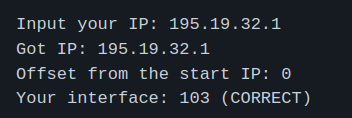
\includegraphics[width=0.5\textwidth]{img/example.png}
	\end{center}
	\caption{Тест программы}
	\label{img:graph1}
\end{figure}
